\newpage
\section{Approach}
\label{sec:Approach}


\begin{figure}[!htbp]
	\centering
	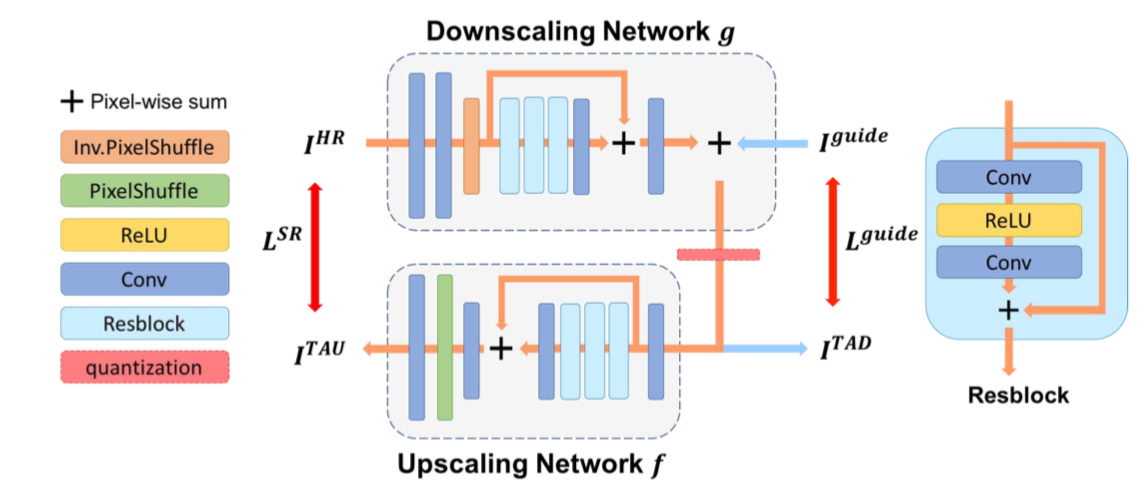
\includegraphics[width=10cm]{figures/tad_overview}
	\caption{Overview of TAID autoencoder network design \cite{TAID}.}
  \label{fig:tad_overview}
\end{figure}


% The objectives of the ``Materials and Methods'' section are the following:
% \begin{itemize}
%  \item \textit{What are tools and methods you used?} Introduce the environment, in which your work has taken place - this can be a software package, a device or a system description. Make sure sufficiently detailed descriptions of the algorithms and concepts (e.g. math) you used shall be placed here.
%  \item \textit{What is your work?} Describe (perhaps in a separate section) the key component of your work, e.g. an algorithm or software framework you have developed.
% \end{itemize}
